\newpage
\section{The Single-Particle Propagator Re-Visited}
\subsection{Mathematical expression for the single-particle Green's function propagator}
The closed mathematical expression for the propagator,$G$, appears usually in one of two forms:
\begin{equation}\begin{aligned}
G\left(k_{2}, k_{1}, t_{2}-t_{1}\right) &=-i\left\langle\Psi_{0}\left|T\left\{c_{k_{2}}\left(t_{2}\right) c^{\dagger}_{k_{1}}\left(t_{1}\right)\right\}\right| \Psi_{0}\right\rangle \\
G\left(\mathrm{r}_{2}, \mathrm{r}_{1}, t_{2}-t_{1}\right) &=-i\left\langle\Psi_{0}\left|T\left\{\psi\left(\mathrm{r}_{2}, t_{2}\right) \psi^{\dagger}\left(\mathrm{r}_{1}, t_{1}\right)\right\}\right| \Psi_{0}\right\rangle
\end{aligned}
\label{sandwitch-defi-G}
\end{equation}
We shall only consider the first form-the second may be analysed in a similar way. First, $\Psi_{0}$ is the exact normalized wave function of the ground state of the interacting $N$ -particle system. The operators $c_{k}(t), c_{k}^{\dagger}(t)$ respectively, destroy and create a particle in state $k$ at time $t .$ More precisely, they are the ordinary $c_{k}, c_{k}^{\dagger}$ transformed to \redp{'Heisenberg picture'}, defined by
\begin{equation}\begin{array}{l}
c^{\dagger}_{k_{1}}\left(t_{1}\right)=e^{+i Ht_{1}} c_{k_{1}} e^{-i H t_{1}} \\
c_{k_{2}}\left(t_{2}\right)=e^{+i Ht_2} c_{k_{2}} e^{-i Ht_{2}}
\end{array}\end{equation}
Finally the Wick time-ordering operator, T, is defined by
\begin{imp}
\begin{equation}
\begin{aligned}
T\left\{A\left(t_{1}\right) B\left(t_{2}\right) \ldots\right\}=&(-1)^{P} \times\begin{varwidth}[t]{\linewidth}operators rearranged so that time\\decreases from left to right, assuming\\no two times are equal,\end{varwidth}\\
&=(-1)^P\times\begin{varwidth}[t]{\linewidth}operators rearranged so all $c^{\dagger}$ 's (or\\ $a^{\dagger}$' s or $b$'s) stand to the left of $c$'s $($ or\\ $a$'s or $\boldsymbol{b}^{\dagger}$ 's ) for the case of equal\\ times)\end{varwidth}
\end{aligned}
\end{equation}
where $P$ is the number of interchanges of operators required to get the operators in the proper time order, starting with the order given in the brackets.
\end{imp}
Thus, 
\begin{equation}\begin{aligned}
T\left\{c_{k_{2}}\left(t_{2}\right) c_{k_{1}}\left(t_{1}\right)\right\} &=c_{k_{2}}\left(t_{2}\right) c^{\dagger}_{k_{1}}\left(t_{1}\right) \text { for } t_{2}>t_{1} \\
&=-c_{k_{1}}^{\dagger}\left(t_{1}\right) c_{k_{2}}\left(t_{2}\right) \text { for } t_{2} \leqslant t_{1}
\end{aligned}\end{equation}
and
\begin{equation}\begin{aligned}
G &=G^{+}\left(k_{2}, k_{1}, t_{2}-t_{1}\right)=-i\left\langle\Psi_{0}\left|c_{k_{2}}\left(t_{2}\right) c^{\dagger}_{k_{1}}\left(t_{1}\right)\right| \Psi_{0}\right\rangle, \quad t_{2}>t_{1} \\
&=G^{-}\left(k_{2}, k_{1}, t_{2}-t_{1}\right)=+i\left\langle\Psi_{0}\left|c^{\dagger}_{k_{1}}\left(t_{1}\right) c_{k_{2}}\left(t_{2}\right)\right| \Psi_{0}\right\rangle, \quad t_{2} \leqslant t_{1}
\end{aligned}\end{equation}
Consider the $t_2>t_1$ case first, we have
\begin{equation}G^{+}=-\underbrace{I\left\langle\Psi_{0}\right| e^{i Ht_{2}} c_{k_{2}}}_{B^{\dagger}} \underbrace{e^{-i H\left(t_{2}-t_{1}\right)} c^{\dagger}_{k_{1}} e^{-i Ht_{1}}\left|\Psi_{0}\right\rangle}_{A}
\label{G+=BA}
\end{equation}
Now \redp{$exp(-iHt)$ is the time development operator}, so that $exp(-iHt_1)|\Psi_0\rangle$ is the ground state at time $t_1$, and $c^{\dagger}_{k_1}exp(-iHt_1)|\Psi_0\rangle$ is the state with one particle in $\phi_{k_1}$ added to the ground state at time $t_1$. Hence $\mathbf{A}$ is the state of the system at time $t_2$ when a particle $\phi_{k_1}$ was added at $t_1$. The $B^{\dagger}$ is
\begin{equation}B^{\dagger}=\overline{c^{\dagger}_{k_{2}} e^{-iH t_{2}} |\Psi_{0}}\rangle\end{equation}
This is \bluep{the complex conjugate of the state with one particle in $\phi_{k_2}$ added to the ground state at time $t_2$.} Hence we obtain
\begin{equation}
    \begin{aligned}
    G^+=B^{\dagger}A&=\text{component of B along A}\\
    &=\begin{varwidth}[t]{\linewidth}
    probability amplitude that the state of the system\\
    at $t_{2},$ when a particle in $\phi_{k_{1}}$ was added to the\\ 
    ground state at $t_{1},$ is the state with one particle in \\
    $\phi_{k_{2}}$ added to the ground state at time $t_{2}$
    \end{varwidth}
    \end{aligned}
\end{equation}
It is a good brain-building exercise to show how (\ref{sandwitch-defi-G}) boils down to the expression for the free propagator (\ref{combined-G0-in-k-t-space}), in the non-interacting case. The non-interacting Hamiltonian and ground state are given by
\begin{equation}H_{0}=\sum_{p} \epsilon_{p} c_{p}^{\dagger} c_{p}, \quad H_{0}\left|\Phi_{0}\right\rangle=\sum_{p<k_{F}} \epsilon_{p}\left|\Phi_{0}\right\rangle, \quad\left|\Phi_{0}\right\rangle=\left|111 \ldots 1_{F} 000 \ldots\right\rangle\end{equation}
Let us calculate just $G_0^+$ setting $t_1=0,t_2=t$:
\begin{equation}G_{0}^{+}(k, t)=-i\left\langle\Phi_{0}\left|e^{+i H_{0}t} c_{k} e^{-iH_{0}t} c_{k}^{\dagger}\right| \Phi_{0}\right\rangle \theta_{t}\end{equation}
In an obvious notation,
\begin{equation}c_{k}^{\dagger}\left|\Phi_{0}\right\rangle=(-1)^{N}\left|\Phi_{0}, 1_{k}\right\rangle \theta_{\epsilon_k-\epsilon_F}\end{equation}
Thus $k$ must be greater than $k_F$. Now
\begin{equation}H_{0}\left|\Phi_{0}, 1_{k}\right\rangle=\sum_{p} \epsilon_{p} c_{p}^{\dagger} c_{p}\left|\Phi_{0}, 1_{k}\right\rangle=\left[\sum_{p<k_{F}} \epsilon_{p}+\epsilon_{k}\right]\left|\Phi_{0} 1_{k}\right\rangle\end{equation}
Thus
\begin{equation}c_{k} e^{-i H_{0} t}\left|\Phi_{0}, 1_{k}\right\rangle=(-1)^{N}\left|\Phi_{0}\right\rangle \exp \left\{-i\left[\sum_{p<k_{F}} \epsilon_{p}+\epsilon_{k}\right] t\right\}\end{equation}
Finally we have
\begin{equation}G_{0}^{+}(k, t)=-i \theta_{\epsilon_k-\epsilon_F} \theta_{t} e^{-i \epsilon_k t}\end{equation}
confirming (\ref{combined-G0-in-k-t-space}). It is now easy to obtain the ground state expectation value of any single-particle operator in terms of the propagator (\ref{one-body-interaction-occ}), thus
\begin{imp}
\begin{equation}\left\langle\Psi_{0}\left|\mathcal{O}^{o c c}\right| \Psi_{0}\right\rangle=-i \sum_{k l} \mathcal{O}_{k l} \lim _{t \rightarrow 0^{-}} G(l, k ; t)\end{equation}
\end{imp}
\subsection{Spectral density function}
The spectral density function is indispensable for analysing the mathematical properties of propagators, especially their \bluep{analytic properties. Secondly, it is extremely convenient to use in many-body calculations which \textbf{involve diagrams containing 'dressed' or 'renormalized' propagators}}. Here we provide a brief introduction to the subject here. More details can be found in Appendix.

The idea is similar to the spectral decomposition of a time-dependent function $f(t)$ into the sum of its components at various frequencies:
\begin{equation}f(t)=\int_{-\infty}^{+\infty} F(\omega) e^{i \omega t} d \omega\end{equation}
where $F(\omega)$ gives the spectrum of $f(t)$. The corresponding expression for the propagator is, for a system with no external potential:
\begin{imp}
\begin{equation}\begin{aligned}
G(\mathbf{k}, t) &=-i \int_{0}^{\infty} d \omega A^{+}(\mathbf{k}, \omega) e^{-i(\omega+\mu) t}, \quad t>0 \\
&=+i \int_{0}^{\infty} d \omega A^{-}(\mathbf{k}, \omega) e^{+i(\omega-\mu) t}, \quad t \leqslant 0
\end{aligned}
\label{G-spectral-density}
\end{equation}
where $\mu$ is the chemical potential:
\begin{equation}
    \mu=\left[\begin{varwidth}[t]{\linewidth}ground state energy\\ of interacting $N$\\ particle system\end{varwidth}\right]-\left[\begin{varwidth}[t]{\linewidth}ground state energy\\ of interacting $N-1$\\ particle system\end{varwidth}\right]=E_0^N-E_0^{N-1}
\end{equation}
\end{imp}
The $\mathbf{A}^{\pm}(\mathbf{k},\omega)$ is the "spectral density function". The Fourier transform of (\ref{G-spectral-density}) yields
\begin{equation}G(\mathbf{k}, \omega)=\int_{0}^{\infty} d \omega^{\prime}\left\{\frac{A^{+}\left(\mathbf{k}, \omega^{\prime}\right)}{\omega-\omega^{\prime}-\mu+i \delta}+\frac{A^{-}(\mathbf{k}, \omega^{\prime})}{\omega^{\prime}+\omega-\mu-i \delta}\right\}
\label{fourier-G-spectral}
\end{equation}
which is the so-called \redp{'Lehmann representation' of the propagator}, especially useful for discussing analytic properties. The spectral density has the important properties that
\begin{equation}\begin{array}{c}
A^{\pm}(\mathbf{k}, \omega) \geqslant 0, \quad \text { real } \\
\int_{0}^{\infty}\left[A^{+}(\mathbf{k}, \omega)+A^{-}(\mathbf{k}, \omega)\right] d \omega=1 \quad\left(^{*} \text { "sum rule"}\right)
\end{array}
\end{equation}
\bluep{For free particles the spectral density is a $\delta-$function:}
\begin{equation}A_{0}^{\pm}(\mathbf{k}, \omega)=\delta\left(\pm \omega-\epsilon_{k}+\mu\right)\end{equation}
For quasi particles, the $\delta-$function gets broadened out and we find the Lorentz form
\begin{equation}A_{\text {quasi }}^{\pm}(\mathbf{k}, \omega)=\frac{1}{\pi} \frac{\left(1 / \tau_{k}\right) Z_{k}}{\left[\omega \mp\left(\epsilon_{k}^{\prime}-\mu\right)\right]^{2}+\left(1 / \tau_{k}\right)^{2}}+D(\mathbf{k}, \omega)\end{equation}
where $D(\mathbf{k},\omega)$ is a correction required so that the sum rule is satisfied. Finally, we note that if (\ref{squeezed-Lorentzian-defi}) is applied to (\ref{fourier-G-spectral}) we obtain the following to calculate $\mathbf{A}^{\pm}$:
\begin{equation}\begin{array}{l}
A^{+}(\mathbf{k}, \omega-\mu)=-\frac{1}{\pi} \operatorname{Im} G(\mathbf{k}, \omega), \quad \omega>\mu \\
A^{-}(\mathbf{k}, \mu-\omega)=+\frac{1}{\pi} \operatorname{Im} G(\mathbf{k}, \omega), \quad \omega<\mu
\end{array}\end{equation}

\subsection{Topology of diagrams}
In order to develop general methods for working with diagrams, we need a systematic way of drawing all graphs in nth order. This will be discussed now.

The method of drawing the diagrams may be greatly simplified if we associate the full propagator, $G=G^-+G^+$ with directed lines instead of just $G^+$ or $G^-$. This is called the "\redp{\textbf{Feynman method}}". Then in the integrals over intermediate times we automatically get $G_{0}\left(t^{\prime}-t\right)=G_{0}^{+}$ when $t^{\prime}>t$ and $G_{0}\left(t^{\prime}-t\right)=G_{0}^{-}$ when $t^{\prime} \leqslant t .$ Thus it is no longer
necessary to draw any hole lines since a directed line is a particle line for $t^{\prime}>t$ and a hole line for $t^{\prime}<t .$ Thus the time order of the dots is no longer important.

Drawing diagrams in the case of mutually interacting fermions with no external potential is considerably more difficult. To get all nth-order Goldstone diagrams, drawn wiggly lines each with vertex dots at both ends, and two fixed points, thus (note that the wiggles may have any vertical position relative to the fixed points). Join all points to each other with directed lines in all linked topologically distinct (in the Goldstone sense) ways such that one line enters and one leaves each vertex point, and a line enters one external point and leaves the other.

To illustrate, a few typical 2nd-order ones are shown in (\ref{typical-2nd-order-diagrams}). Many of the diagrams in (\ref{typical-2nd-order-diagrams}) can be eliminated. First \bluep{because of conservation of momentum, graphs (b),(d),(h),(i),(j),(l) have a particle and a hole both in the same momentum state. But this is impossible in particle-hole formalism}. 
\begin{mybox}
Such graphs are called 'anomalous' or 'momentum non-conserving'. They do give a contribution when the system is non-isotropic, e.g. external field present, or at finite temperatures.
\end{mybox}
Second, it we agree to use the Feynman convention in which the full $G$ is associated with each line and time order has no significance, then \bluep{$(f)\equiv(e),(g)\equiv(k)$}. Hence the only survivors are (\ref{typical-2nd-order-diagrams-2}) or (\ref{typical-2nd-order-diagrams-3}), where (\ref{typical-2nd-order-diagrams-3}) is another conventional way of drawing the diagrams (\bluep{obtained by making the diagrams out of rubber bands and pulling at top and bottom until the main line is straight}). Equations (\ref{typical-2nd-order-diagrams-2}) and (\ref{typical-2nd-order-diagrams-3}) are topologically equivalent in the Feynman sense.
\begin{equation}
    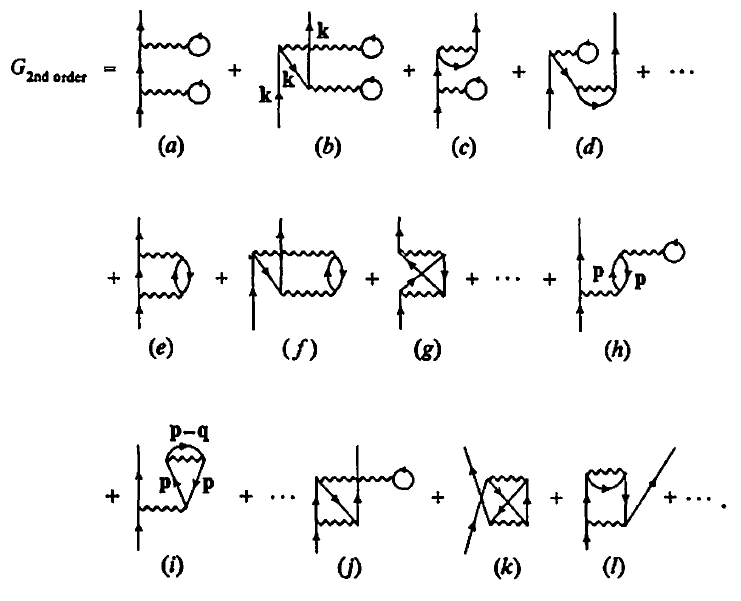
\includegraphics[width=0.8\textwidth]{screenshots/typical-2nd-order-diagrams.PNG}
    \label{typical-2nd-order-diagrams}
\end{equation}
\begin{equation}
    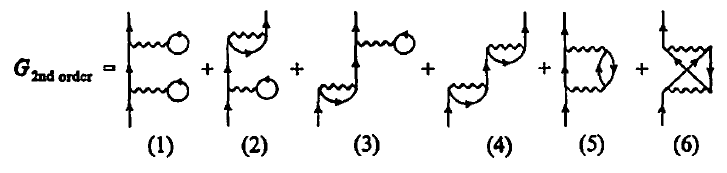
\includegraphics[width=0.8\textwidth]{screenshots/typical-2nd-order-diagrams-2.PNG}
    \label{typical-2nd-order-diagrams-2}
\end{equation}
\begin{equation}
    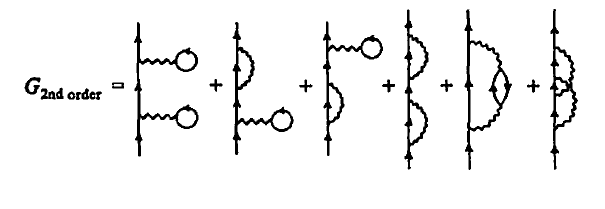
\includegraphics[width=0.8\textwidth]{screenshots/typical-2nd-order-diagrams-3.PNG}
    \label{typical-2nd-order-diagrams-3}
\end{equation}
Let us evaluate a typical second-order diagram using the Feynman method.
\begin{equation}
    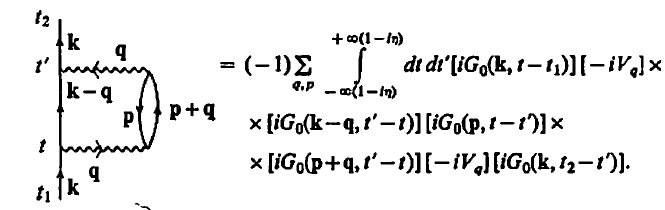
\includegraphics[width=0.8\textwidth]{screenshots/typical-feynman-diagrams-to-integral.PNG}
    \label{typical-feynman-diagrams-to-integral}
\end{equation}
Note that \redp{the order of the times in G is always: time at end of directed line minus time at beginning.} The Fourier transform of (\ref{typical-feynman-diagrams-to-integral}) is
\begin{equation}
    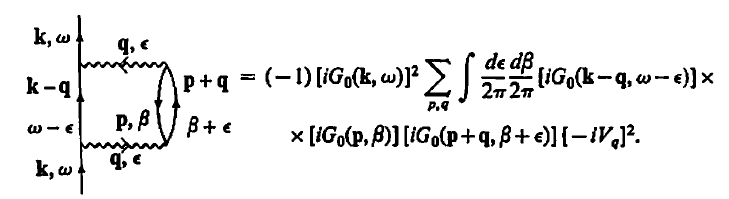
\includegraphics[width=0.8\textwidth]{screenshots/typical-feynman-diagrams-to-integral-fourier.PNG}
\end{equation}
It is seen that the frequencies, $\omega, \epsilon, \beta,$ etc., are conserved at the vertices, just like the momentum. This comes about because of the appearance of $\delta$ -functions similar to the $2 \pi \delta\left(\omega^{\prime}-\omega\right)$ when the transform is carried out. \bluep{\textbf{The "$2\pi$" in $\frac{d\epsilon}{2\pi}$ comes from Fourier transformation too.}}

One more thing, We can avoid treating the 'non-propagating' lines as a special case by including a convergence factor $exp(i\omega 0^+)$ when translating these lines into functions, where $0^+$ is a positive infinitesimal such that $0^{+} \times \infty=\infty$, thus
\begin{imp}
\begin{equation}
    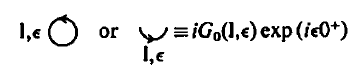
\includegraphics[width=0.8\textwidth]{screenshots/non-propagating-treatment.PNG}
\end{equation}
Hence the integral over the intermediate frequency $\epsilon$ gives:
\begin{equation}
\int_{-\infty}^{+\infty} \frac{d \epsilon}{2 \pi} \frac{i e^{i \epsilon 0^+}}{\epsilon-\epsilon_{l}+i \delta_l}=\begin{aligned}
-1 & \text { for } \quad l<k_{F} \\
0 & \text { for } \quad l>k_{F}
\end{aligned}\end{equation}
where $\delta_l=-\delta$ when $l<k_F$. The integral is done by contour residues theorem. The contour is closed in the upper half-complex-plane where the convergence factor makes the arc integral vanish.
\end{imp}
Thus, for example
$$
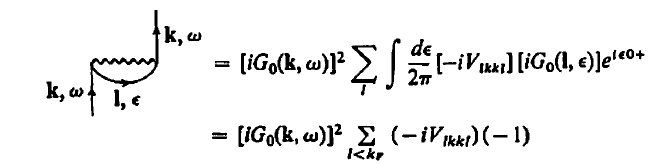
\includegraphics[width=0.8\textwidth]{screenshots/non-propagating-treatment-example.PNG}
$$

\subsection{Diagram rules for single-particle propagator}
We have now reached the point where we can present in summary form the rules for drawing and evaluating the type of graphs which will be used in the next two chapters. These are the diagrams describing a system of mutually interacting fermions with no external field and they will always be drawn in $(\mathbf{k},\omega)$-space, using the Feynman method. The rules are:

\begin{easylist}
\NewList
@ In nth order, drawn wiggly lines with vertex dots and two external points

@ Join all vertex dots and external points to each other with directed lines in all linked topologically distinct (in the Feynman sense) ways, with one line entering and one leaving each vertex dot and a line entering one external point and leaving the other. Two diagrams are topologically distinct if they are visualized as made of rubber bands, and one cannot be deformed into the other.

@ Label each line and wiggle with a momentum, k (short for $\mathbf{k}, \sigma,$ where $\boldsymbol{\sigma}=\operatorname{spin}),$ and frequency $\omega,$ such that the sum of momenta (and frequencies) entering each vertex = sum of those leaving. Eliminate all 'anomalous' or 'momentum-non-conserving' diagrams, i.e., which have a hole and a particle in the same state.

@ Evaluate graphs by means of the dictionary in the following table
\end{easylist}
\begin{table}[H]
    \centering
    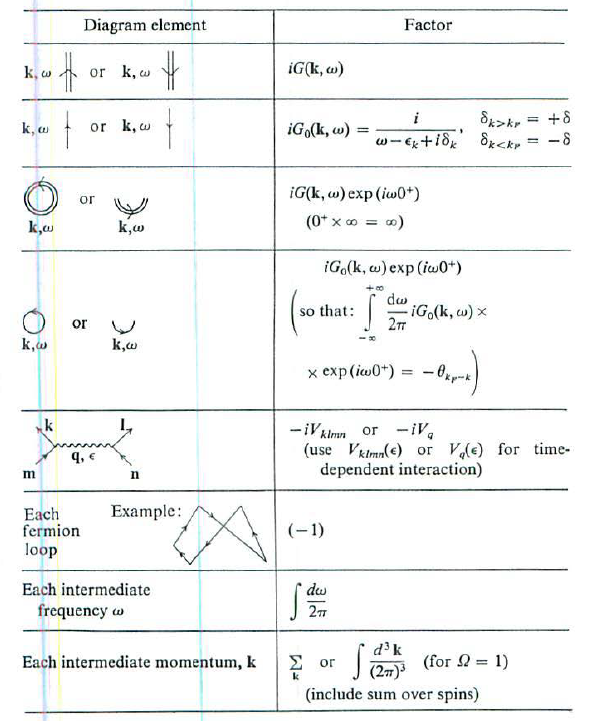
\includegraphics[width=0.6\textwidth]{screenshots/table-feynman-diagram-rules.PNG}
    \caption{Diagram dictionary for interacting many-fermion system with
no external potential (Feynman method)}
    \label{tab:feynman-diagram-rules}
\end{table}
Some physicists use abbreviated diagram in which the interaction wiggles are compressed to points or little squares. Thus, for example
\begin{equation}
    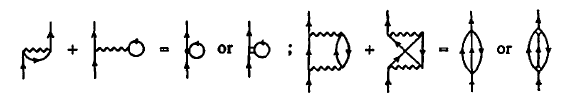
\includegraphics[width=0.8\textwidth]{screenshots/Hugenholtz-diagrams.PNG}
\end{equation}
Those drawn with points are called "Hugenholtz diagrams", while those with squares are "Abrikosov diagrams".

\subsection{Modified propagator formallsm using chemical potential,\texorpdfstring{$\mu$}{TEXT}}
The formalism just described can be somewhat inconvenient in actual calculations because, unless special precautions are taken, it may produce approximations for $G$ which yield the wrong total number of particles for the system.

In order to understand this, let us first derive the relation between the propagator $G$ and the total particle number N. The quantity N is the expectation value of the total number  operator $2\sum_k c^{\dagger}_k c_k$(factor of 2 for spin) in the interacting ground state:
\begin{equation}N=\left\langle\Psi_{0}\left|2 \sum_{k} c^{\dagger}_{k} c_{k}\right| \Psi_{0}\right\rangle=2 \sum_{k}\left\langle\Psi_{0}\left|c^{\dagger}_{k} c_{k}\right| \Psi_{0}\right\rangle\end{equation}
The summand is easily expressed in terms of $G(k_2,k_1,t_2-t_1)$ by setting $t_2=t,t_1=0,k_1=k_2=k$, then letting t approach zero from the left. This yields
\begin{equation}N=2 \sum_{k}(-i) \times \lim _{t \rightarrow 0^{-}} G(k, t)=-2 i \lim _{t \rightarrow 0^{-}} \int \frac{d^{3} \mathbf{k}}{(2 \pi)^{3}} \int \frac{d \omega}{2 \pi} G(\mathbf{k}, \omega) e^{-i \omega t}
\label{N-G-relation}
\end{equation}
which is the desired relation.

Imagine that we calculate an approximate G for the system by a partial summation over some types of diagrams in 
\begin{equation}
    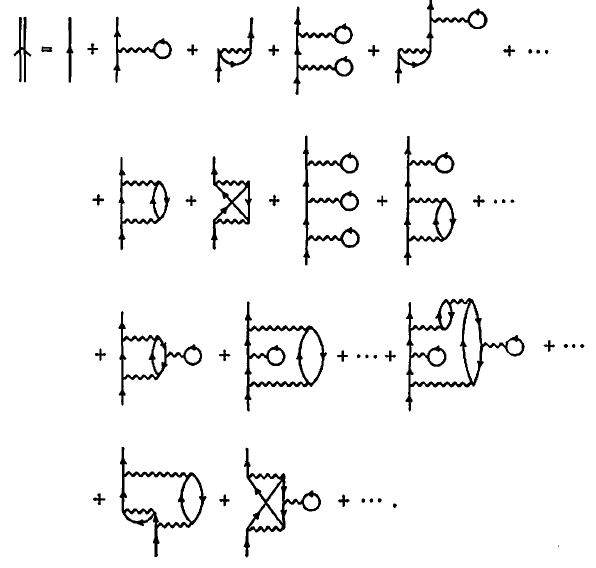
\includegraphics[width=0.8\textwidth]{screenshots/single-propagator-feynman-method.PNG}
    \label{single-propagator-feynman-method}
\end{equation}
and then place this G in (\ref{N-G-relation}) to check and see if it yields $N=N_0$. Evidently, $G$ will be a function of $N_0$, because each $G_0$ entering the calculation of $G$(approx.) depends on $k_F$, and $k_F$ is related to $N_0$ by
\begin{equation}N_{0}=2 \sum_{k<k_{P}} 1=\frac{2}{(2 \pi)^{3}} \int_{k<k=} d^{3} \mathbf{k}=k_{F}^{3} / 3 \pi^{2}, \quad \text { or } \quad k_{F}=\left(3 \pi^{2} N_{0}\right)^{1/3}\end{equation}
Note that the Fermi energy is
\begin{equation}c_{F}=k_{F}^{2} / 2 m=\frac{\left(3 \pi^{2} N_{0}\right)^{2/3}}{2 m}\end{equation}
\bluep{Hence N will be function of $N_0$. But, since $G$ is only approximate, there is no guarantee that $N$ will equal $N_0$}.

It is simple to remove this difficulty by slightly modify the formalism. The method of doing this is to \redp{use the "grand canonical ensemble" at zero temperature. In this method we no longer regard the system as isolated, with definite particle number $N_0$, but instead put it in contact with a particle reservior, so that it can gain or lose particles. Thus, particle number, N is variable throughout the calculation.} The chemical potential of system, $\mu$ is fixed but unknown; its value is determined at the end of the calculation by setting the total particle number equal to $N_0$.
\begin{imp}
The modified Hamiltonian for this case is
\begin{equation}H^{\prime}=H-\mu N=H_{0}^{\prime}+H_{1}\end{equation}
where
\begin{equation}\begin{aligned}
&H_{0}^{\prime}=\sum_{k}\left(\epsilon_{k}-\mu\right) c_{k}^{\dagger} c_{k}\\
&H_{1}=\frac{1}{2} \sum_{k l m n} V_{k l m n} c_{l}^{\dagger} c_{k}^{\dagger} c_{m} c_{n}
\end{aligned}\end{equation}
where N is the total particle number operator.
\end{imp}
The ground state of the modified unperturbed Hamiltonian, $H^{\prime}_{0},$ is obtained by selecting that number of particles, and that way of filling the energy levels which minimizes the energy. \textbf{\redp{It is easily seen that this means all levels filled up to $\epsilon_{k}=\mu, \text { i.e., up to } k_{F}^{\mu}=\sqrt{( 2 m \mu)}$}} The corresponding particle number is $N=\left(3 \pi^{2}\right)^{-1} \times(2 m \mu)^{3/2} .$ The free propagator for $H_{0}^{\prime}$ is
\begin{equation}G_{0}^{\mu}(\mathbf{k}, \omega)=\frac{1}{\omega-\left(\epsilon_{k}-\mu\right)+i \delta_{k}^{\mu}}, \quad \delta_{k}^{\mu}=\left\{\begin{array}{ll}
+\delta & \text { for } \epsilon_{k}>\mu \\
-\delta & \text { for } \epsilon_{k}<\mu
\end{array}\right.\end{equation}
It will be convenient to define a new $\omega$ such that $\omega_{\text {new }} \equiv \omega+\mu .$ In addition, in order to get the correct result when we do self-consistent Hartrec-Fock, it is necessary to re-write the infinitesimal in the form $i \operatorname{sign}(\omega-\mu) \delta$ or $i(\omega-\mu) \delta$ for short, where $\omega \equiv \omega_{\text {new }} .$ These two changes yield $\left(\omega \equiv \omega_{\text {new }}\right)$
\begin{equation}G_{0}^{\mu}(\mathbf{k}, \omega)=\frac{1}{\omega-\epsilon_{k}+i(\omega-\mu) \delta}
\label{G-0-mu}
\end{equation}
Now $N$ becomes a function of $\mu$. If $\mu$ is now determined by setting
\begin{equation}
N(\mu)=N_0
\label{N=N-0}
\end{equation}
we guarantee that $G$(approx.) yields the correct number of particles. Using (\ref{N-G-relation}), (\ref{G-0-mu}), and (\ref{N=N-0}), and ignoring interactions we have:
\begin{equation}N(\mu)=\frac{\left(k_{P}^{\mu}\right)^{3}}{(3 \pi)^{2}}=\frac{(2 m \mu)^{3/2}}{3 \pi^{2}}=N_{0}
\label{N0-kF-relation}
\end{equation}
so that $\mu=\epsilon_F$.